\subsection{IFIT Subcellular Localisation During Interferon Induction and RSV Infection} \label{subsec:IFIT Subcellular Localisation During Interferon INduction and RSV Infection}
put antibody validation wbs

compare and contrast to the info in databases and papers

% introduction to ib stuff from my study
write about ib size statistics from my analysis

\begin{figure}
    \centering
    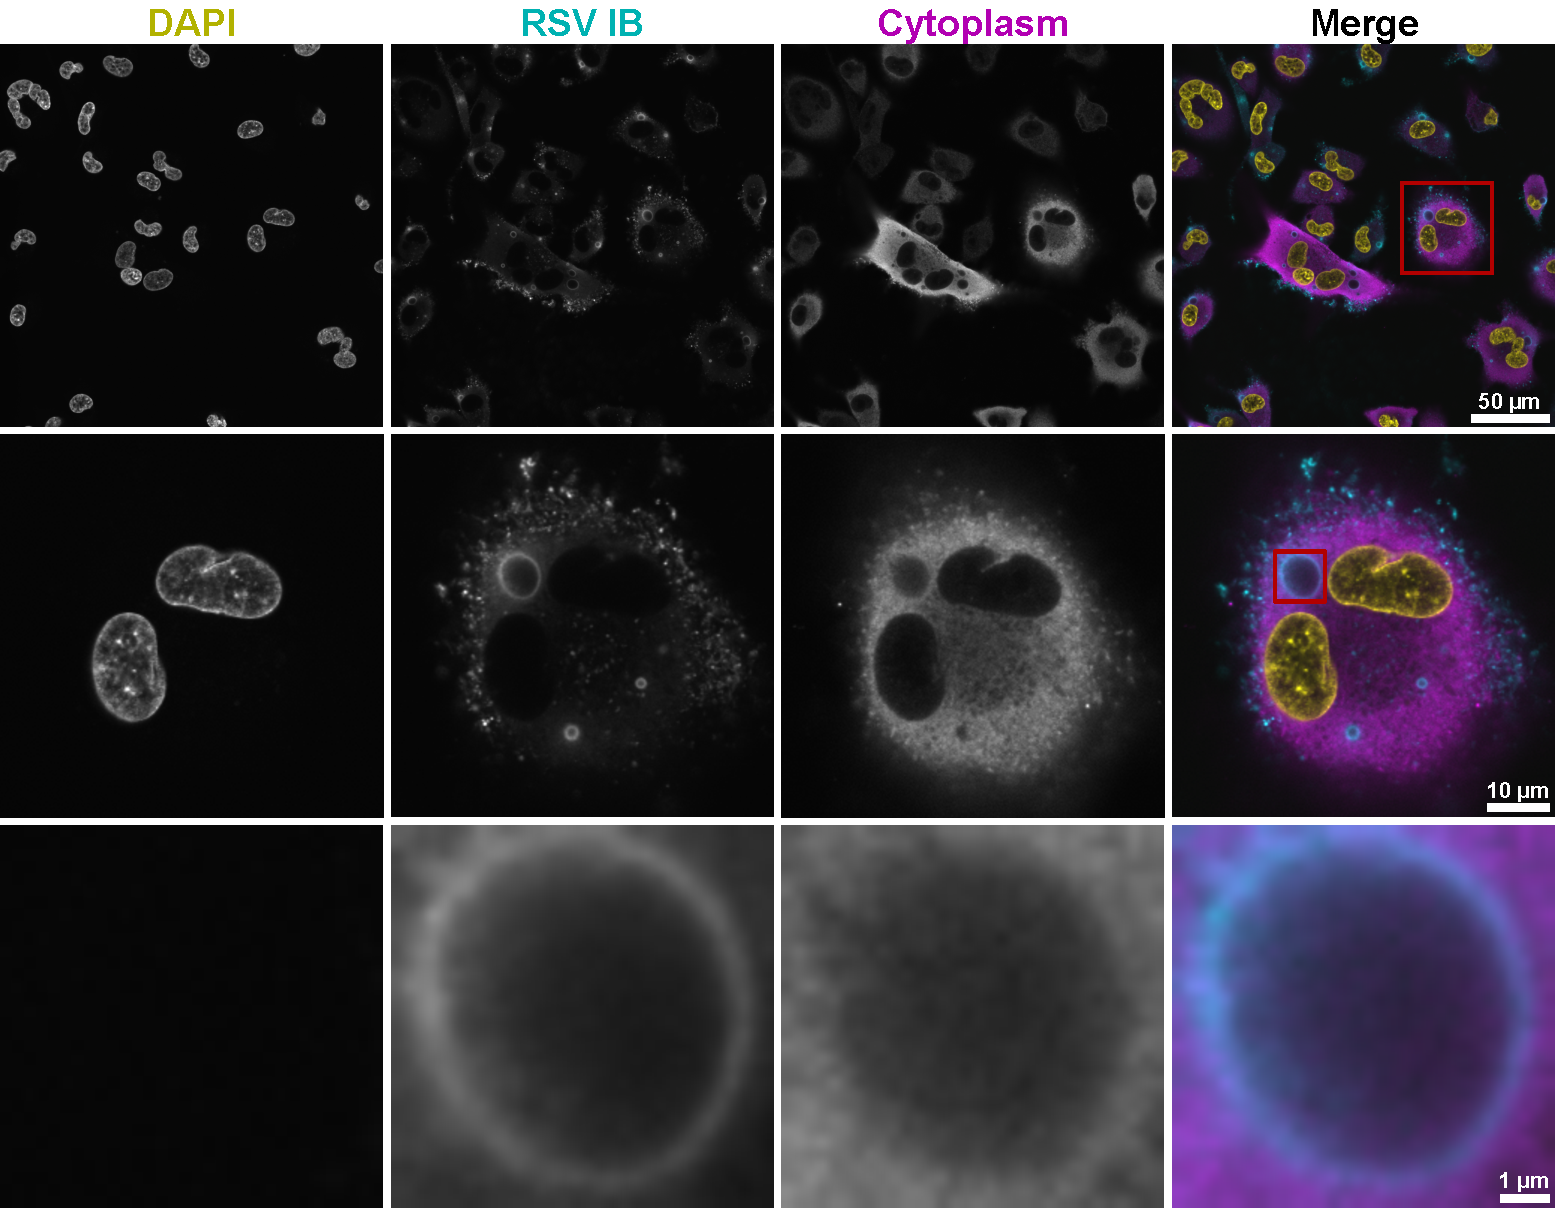
\includegraphics[width=1\linewidth]{09. Chapter 4/Figs/01. Localisation introduction/01. IB-zooms.pdf}
    \caption[Inclusion Bodies Within RSV Infected Cells: Zoom Sequence.]{\textbf{Inclusion Bodies Within RSV Infected Cells: Zoom Sequence.} A represerenative image of RSV infected cells detected using confocal microscopy. Cellular nuclei were stained with DAPI and are shown in yellow; RSV inclusion bodies are shown in cyan; and the cytoplasm is shown in magenta. Figure highlights a zoom sequence from a population of cells, into a single syncytia view, with lastly focusing at one individual inclusion body.}
    \label{fig:Inclusion Bodies Within RSV Infected Cells: Zoom Sequence}
\end{figure}


\begin{figure}
    \begin{subfigure}{0.5\textwidth}
        \caption{}
        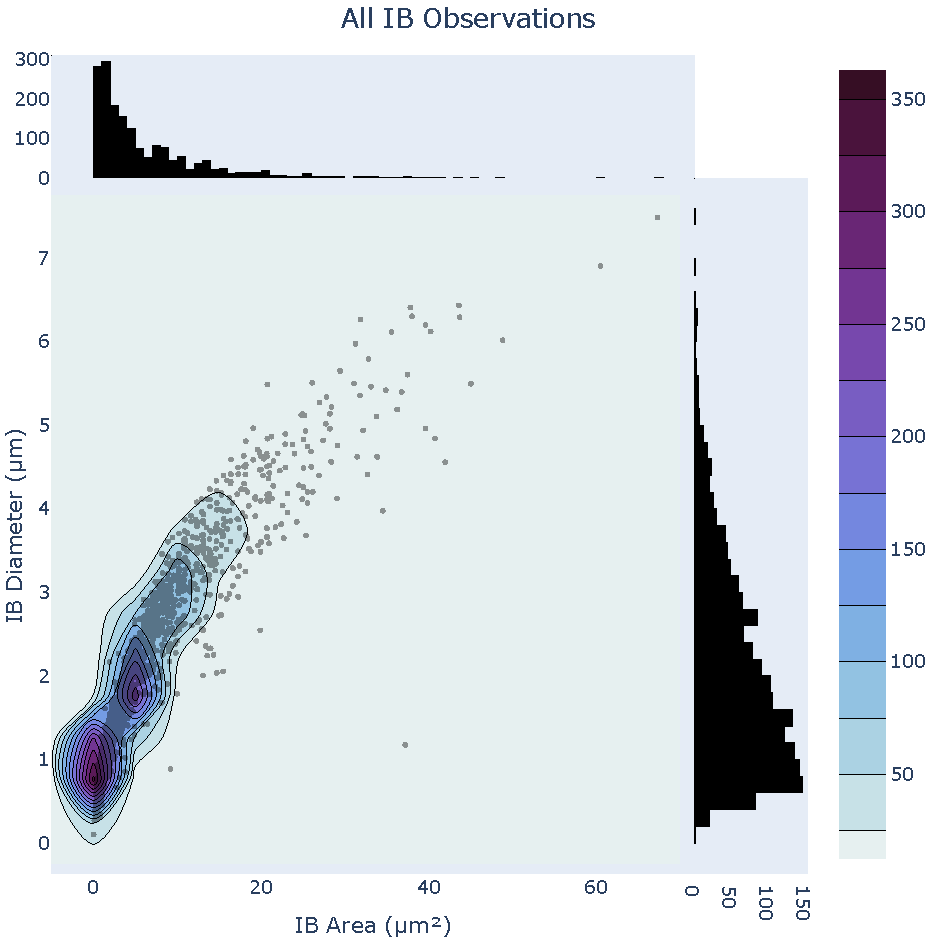
\includegraphics[width=\textwidth]{09. Chapter 4/Figs/01. Localisation introduction/02. heatmap_all.pdf} 
    \end{subfigure}
    \hfill
    \begin{subfigure}{0.5\textwidth}
        \caption{}
        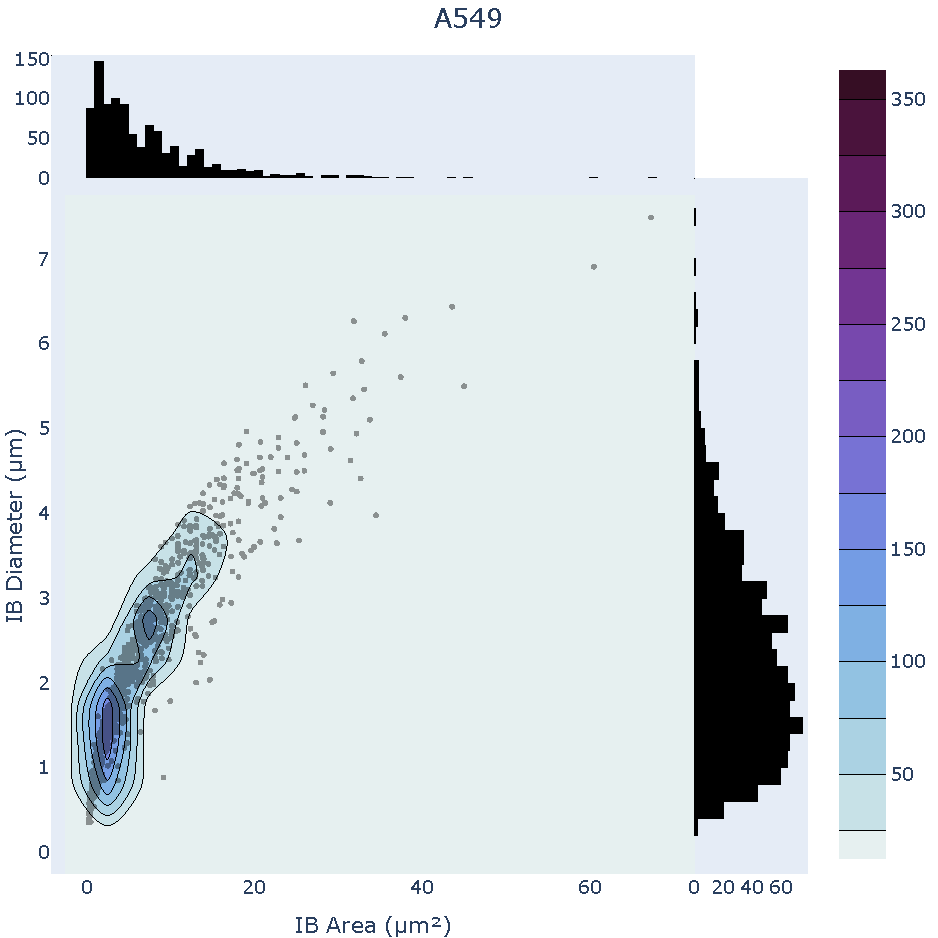
\includegraphics[width=\textwidth]{09. Chapter 4/Figs/01. Localisation introduction/03. heatmap_a549.pdf}
    \end{subfigure}

    \medskip
    \begin{subfigure}{0.5\textwidth}
        \caption{}
        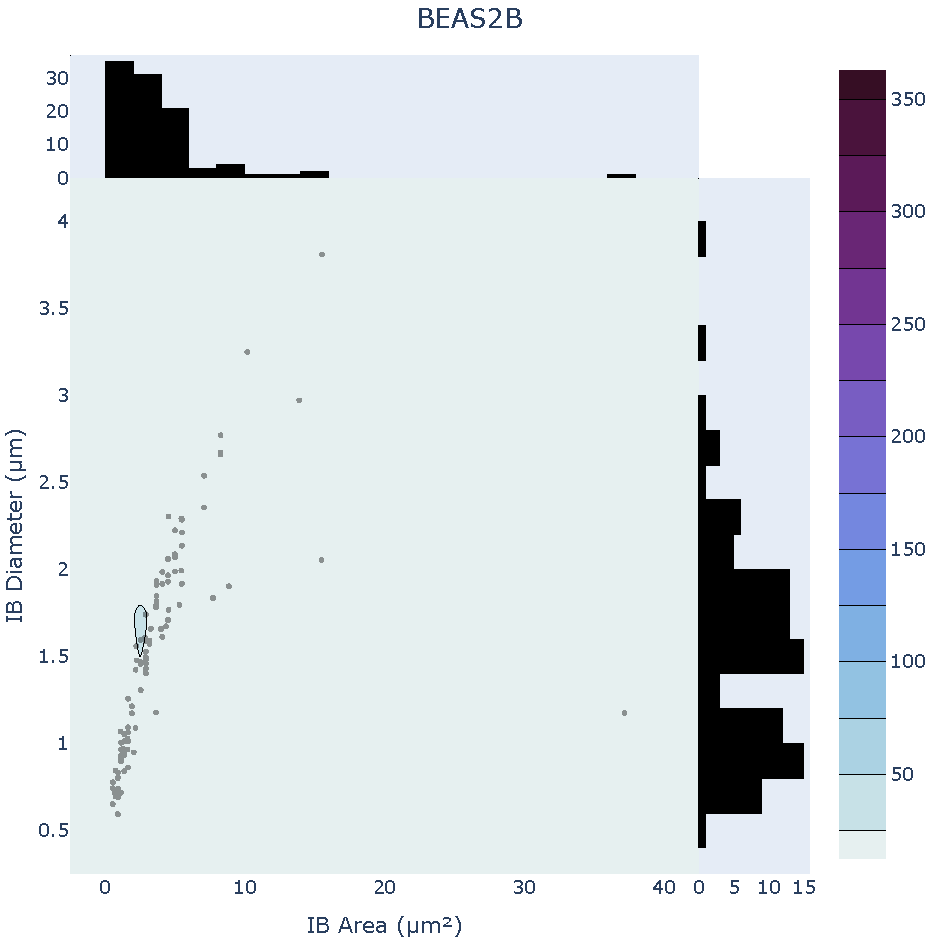
\includegraphics[width=\textwidth]{09. Chapter 4/Figs/01. Localisation introduction/04. heatmap_beas2b.pdf} 
    \end{subfigure}
    \hfill
    \begin{subfigure}{0.5\textwidth}
        \caption{}
        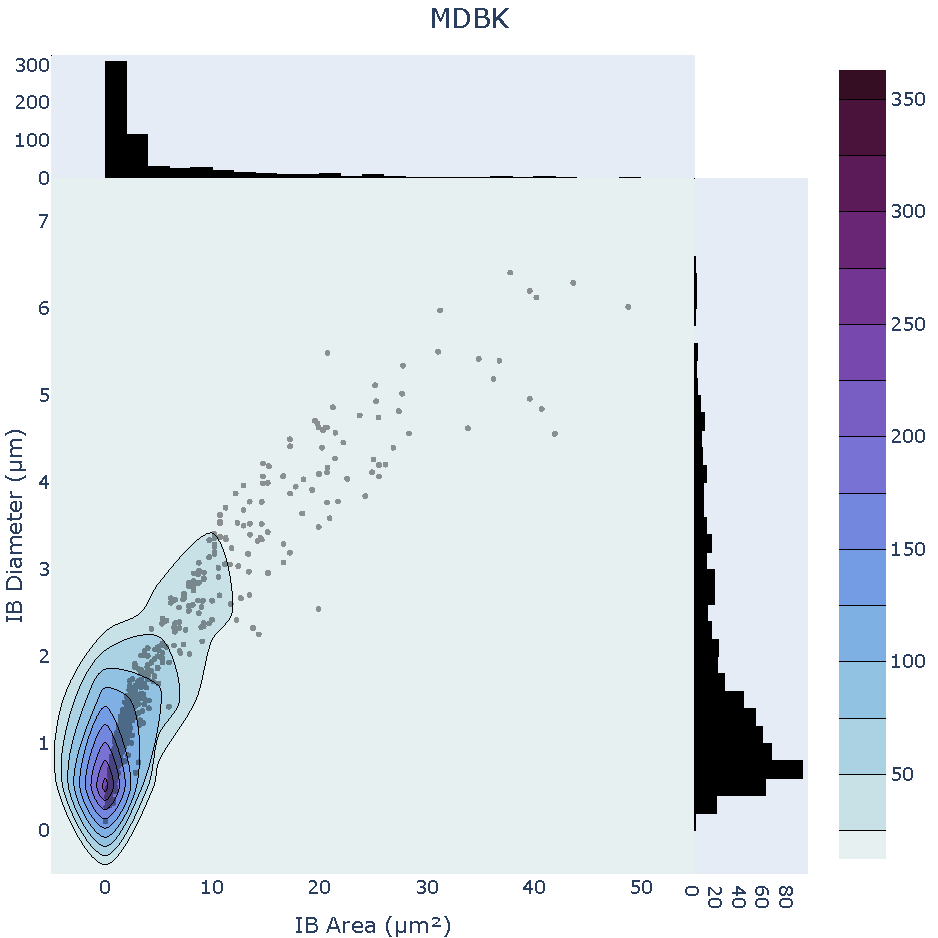
\includegraphics[width=\textwidth]{09. Chapter 4/Figs/01. Localisation introduction/05. heatmap_mdbk.pdf} 
    \end{subfigure}
    
    \caption[Size Characterization of Inclusion Bodies Across Different Cell Lines.]{\textbf{Size Characterization of Inclusion Bodies Across Different Cell Lines.} TThis figure presents the relationship between the measured area (\(\mu m^2\)) and diameter (\(\mu m\)) of individual inclusion bodies (IBs) as observed within the scope of this study. Additionally, the figure includes distinct population distributions depicted alongside the plots, representing (a) the aggregate of 1727 observations of IBs across all individual cell lines, (b) 1008 observations from the A549 cell line, (c) 99 observations from the BEAS2B cell line, and (d) 620 observations from the MDBK cell line. Contour plots are incorporated to elucidate the underlying density of individual IBs within the plots.}
    \label{fig:Size Characterization of Inclusion Bodies Across Different Cell Lines}
    
\end{figure}


% human stuff
Asdfasfsdfasdf \newline
IF Mock | INF | Infection \newline
A549 BEAS2B

Merge pictures of clusters of cells looking at changes between subcellular localisation and a clear increase in mean intensity. Graphs show mean intensity changes from all cells imaged.

\begin{figure}
    \centering
    \includegraphics[width=1\linewidth]{09. Chapter 4/Figs/01. Localisation introduction/06. a549 merges.pdf}
    \caption[A549 localisation mergers.]{\textbf{A549 localisation mergers.} Nascent bovine IFIT1 in the context of bRSV infection has been observed to localise with the respect of IB in three distinct spaces. We observed it either concentrated inside the central point of the IB structure, while having reduced signal on the inner IB edge, compared to the cytoplasm (top and bottom panels), being excluded from the IB structure (3rd panel), or colocalising on the inner edge of the IB structure while having reduced signal in the middle of the structure compared to cytoplasm, or the edge staining (2nd panel).}
    \label{fig:A549 localisation mergers.}
\end{figure}


\begin{figure}
    \centering
    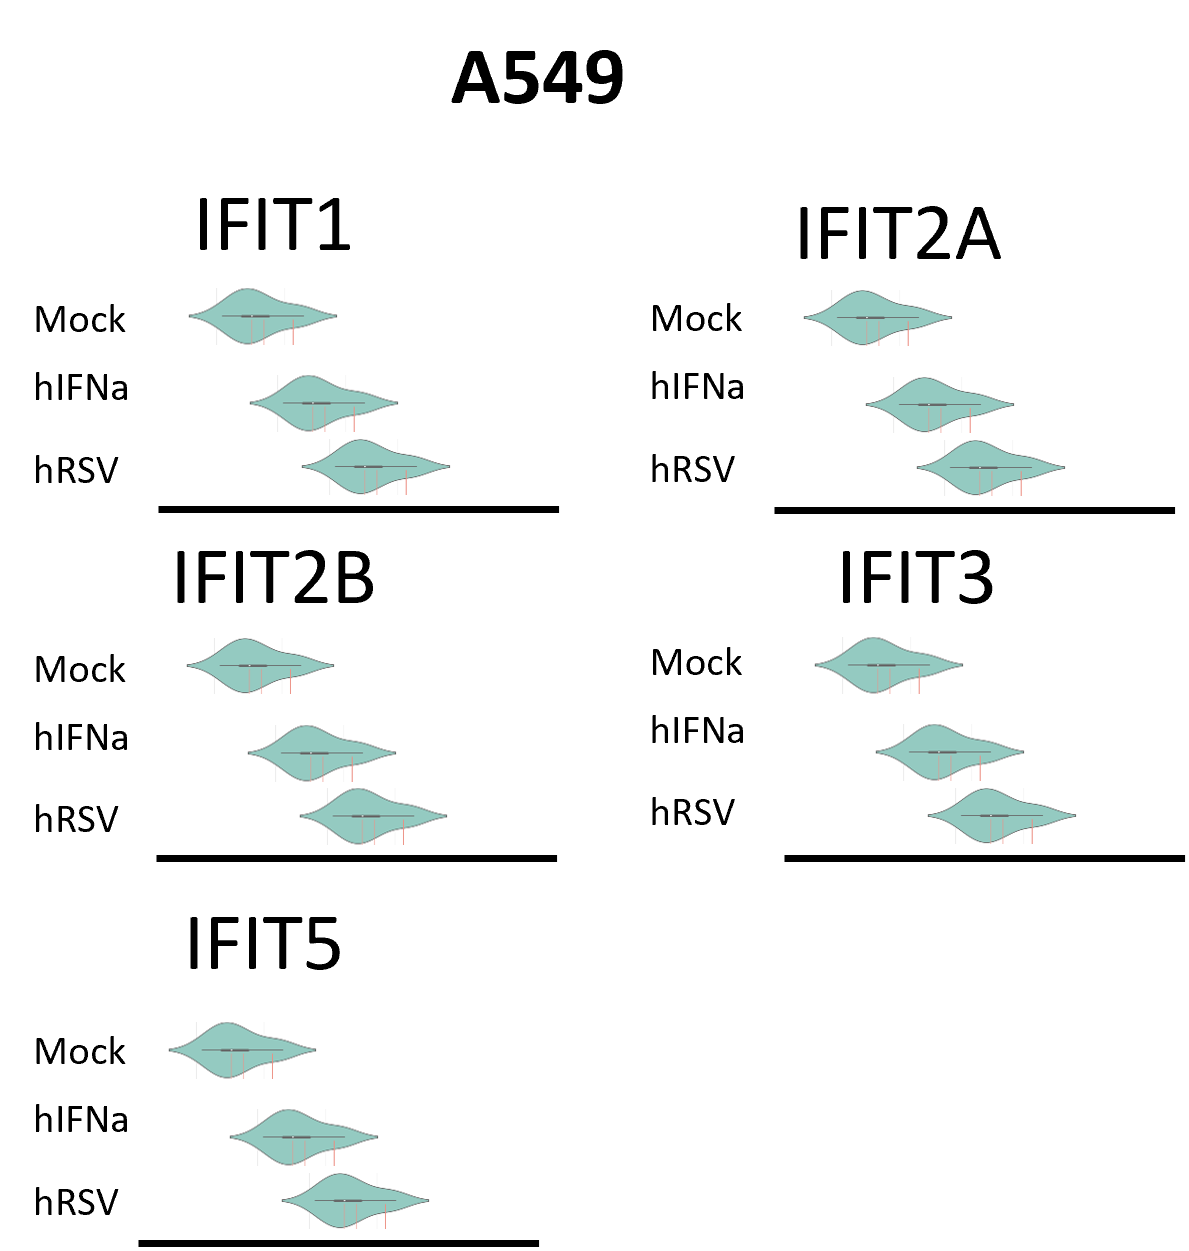
\includegraphics[width=1\linewidth]{09. Chapter 4/Figs/01. Localisation introduction/07. a549 plots.png}
    \caption[A549 localisation plots.]{\textbf{A549 localisation plots.} Nascent bovine IFIT1 in the context of bRSV infection has been observed to localise with the respect of IB in three distinct spaces. We observed it either concentrated inside the central point of the IB structure, while having reduced signal on the inner IB edge, compared to the cytoplasm (top and bottom panels), being excluded from the IB structure (3rd panel), or colocalising on the inner edge of the IB structure while having reduced signal in the middle of the structure compared to cytoplasm, or the edge staining (2nd panel).}
    \label{fig:A549 localisation plots.}
\end{figure}


% bovine stuff
Asdfasfsdfasdf \newline
IF Mock | INF | Infection \newline
MDBK BT

Merge pictures of clusters of cells looking at changes between subcellular localisation and a clear increase in mean intensity. Graphs show mean intensity changes from all cells imaged.

\begin{figure}
    \centering
    \includegraphics[width=1\linewidth]{09. Chapter 4/Figs/01. Localisation introduction/08. mdbk-merges-test.pdf}
    \caption[MDBK localisation mergers.]{\textbf{MDBK localisation mergers.} Nascent bovine IFIT1 in the context of bRSV infection has been observed to localise with the respect of IB in three distinct spaces. We observed it either concentrated inside the central point of the IB structure, while having reduced signal on the inner IB edge, compared to the cytoplasm (top and bottom panels), being excluded from the IB structure (3rd panel), or colocalising on the inner edge of the IB structure while having reduced signal in the middle of the structure compared to cytoplasm, or the edge staining (2nd panel).}
    \label{fig:MDBK localisation mergers}
\end{figure}


\begin{figure}
    \centering
    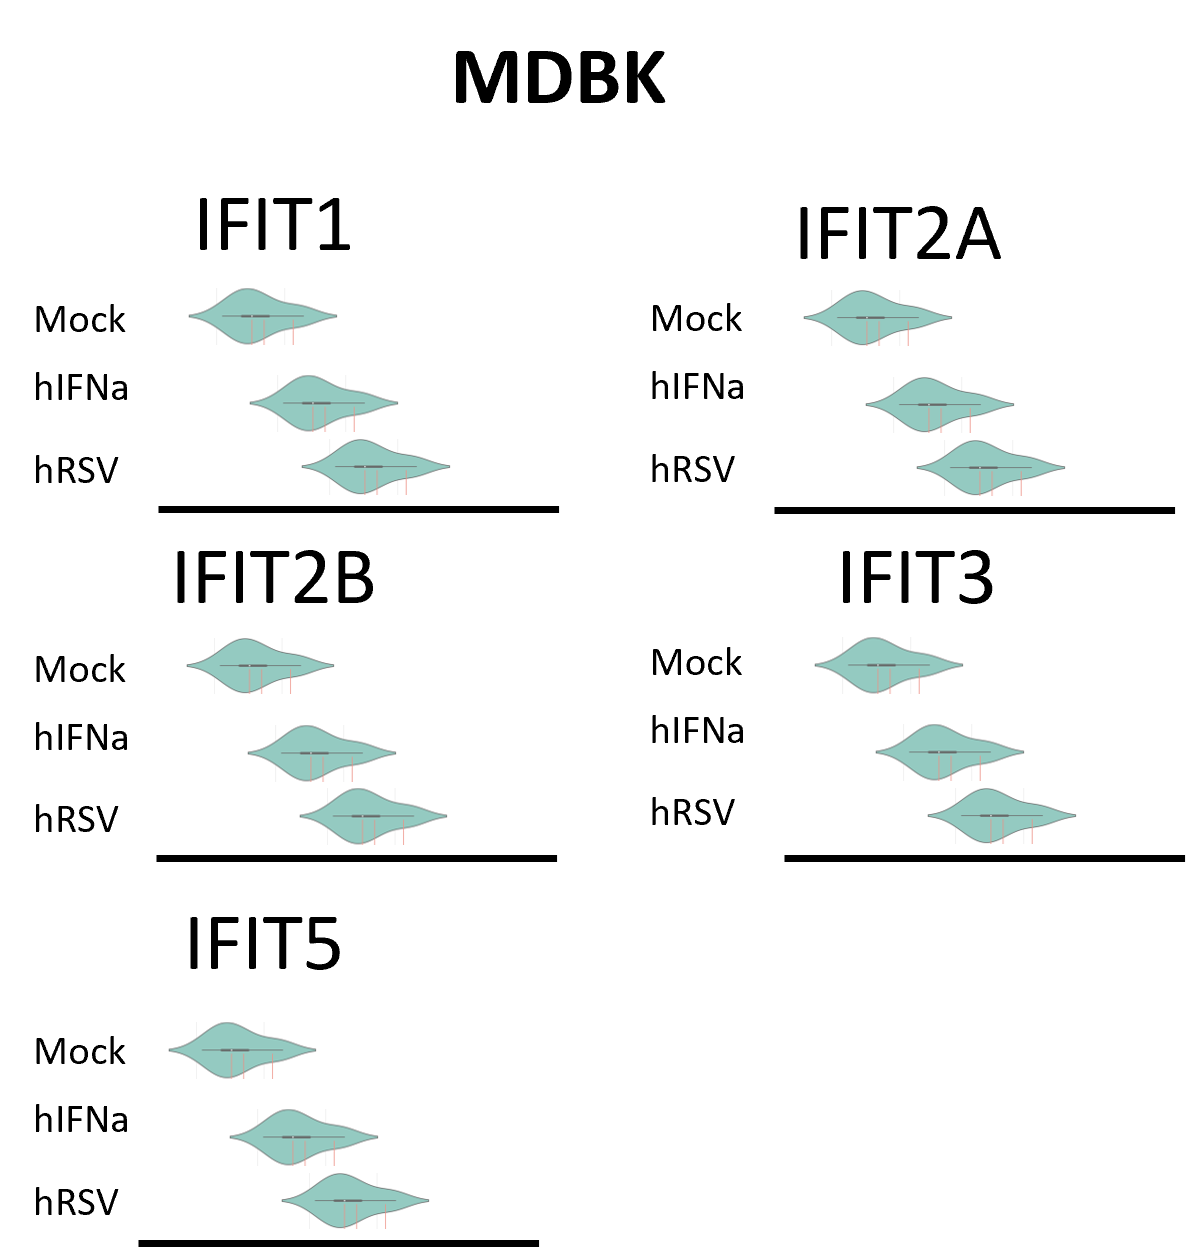
\includegraphics[width=1\linewidth]{09. Chapter 4/Figs/01. Localisation introduction/09. mdbk plots.png}
    \caption[MDBK localisation plots.]{\textbf{MDBK localisation plots.} Nascent bovine IFIT1 in the context of bRSV infection has been observed to localise with the respect of IB in three distinct spaces. We observed it either concentrated inside the central point of the IB structure, while having reduced signal on the inner IB edge, compared to the cytoplasm (top and bottom panels), being excluded from the IB structure (3rd panel), or colocalising on the inner edge of the IB structure while having reduced signal in the middle of the structure compared to cytoplasm, or the edge staining (2nd panel).}
    \label{fig:MDBK localisation plots}
\end{figure}
